\documentclass[12pt]{article}
\usepackage[a4paper, total={7.5in, 11in}]{geometry}
%\usepackage{array}
\usepackage{graphicx, subfig, wrapfig, fancyhdr, lastpage, multicol ,color,arydshln,makecell, tcolorbox}
\newcommand\headerMe[2]{\noindent{}#1\hfill#2}
\usepackage[mathscr]{euscript}
\usepackage{tabularray}

\setlength{\columnseprule}{1pt}
\def\columnseprulecolor{\color{blue}}


\pagestyle{fancy}
\fancyhf{}

\cfoot{ \vspace{-0.8cm}\em{Page \thepage \hspace{1pt} / \pageref{LastPage}}}
\begin{document}

\headerMe{Royaume du Maroc}{année scolaire \emph{2022-2023}}\\
\headerMe{Ministère de l'Éducation nationale, }{  }\\
\headerMe{du Préscolaire et des Sports}{Établissement : \emph{Lycée SKHOR qualifiant}}\\
%\vspace{-1cm}
\begin{center}
%Devoir Surveillé  N°1 \\
    2ème année baccalauréat Sciences physiques\\
%Durée 2h00
    \vspace{.2cm}
\hrulefill
\Large{--Propagation des ondes--}
\hrulefill\\

    %\emph{Les deux parties sont indépendantes}
\end{center}
%end Headerss------------------------
%__________________Chimie ______________________-
%%%%%%%+_+_+_+_+_+_+_+_+_Partie1

 \section*{L'indicateur de vitesse (CINÉMOMÈTRE) \dotfill (2,5 POINTS)  }
%\begin{wrapfigure}{r}{0.16\textwidth}
	%\vspace{-1.2cm}
%\begin{center}
  %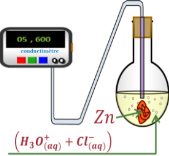
\includegraphics[width=0.16\textwidth]{./img/chimie01.png}
%\end{center}
%\end{wrapfigure}

 \emph{Les dispositifs de mesure de vitesse sont généralement appelés cinémomètres.Les cinémomètres les plus communs peuvent être répartis en deux catégories : les cinémomètres Doppler et \underline{les cinémomètres LASER.}}

 \emph{Cet exercice s’intéresse à certains aspects du fonctionnement et de l’utilisation du cinémomètre LASER}
 \begin{tcolorbox}
Le principe de la mesure de vitesse grâce à cet instrument est basé sur une mesure de la distance
séparant la "cible" du cinémomètre laser. On mesure le temps mis par une impulsion laser pour
atteindre la "cible" visée et revenir au cinémomètre après réflexion. Un compteur électronique de
temps est déclenché lorsque l’impulsion est émise par le laser et arrêté lorsque l’impulsion "retour" est détectée. Connaissant la durée d’un aller-retour ainsi que la vitesse de la lumière, on
en déduit la distance laser-cible. Pour connaître la vitesse de la "cible", il suffit de répéter le
processus de mesure de distance à des intervalles de temps fixes. 
\end{tcolorbox}

\textbf{Données : }
\begin{itemize}
	\item Célérité de la lumière dans le vide :  $c=3,00.10^{8}m.s^{-1}$
\end{itemize}

\textbf{1. Ondes mécaniques et lumineuses : }

\begin{tabular}{c|l}
	0,25  & \makecell[l]{\textbf{1.1. }Définir une onde mécanique. }\\
	0,25  & \makecell[l]{\textbf{1.2. }Le son est une onde longitudinale?Justifier votre réponse.
 }\\

 0,25  & \makecell[l]{\textbf{1.3. }La lumière est-elle une onde mécanique ? Justifier votre réponse.
 }\\

\end{tabular}

\textbf{2. Mesure de la vitesse d’un véhicule }

Le cinémomètre émet des impulsions laser à intervalles de temps réguliers de valeur
$T = 1,80 ms$ en direction d’un véhicule se rapprochant.
Lors de la première émission, le véhicule se trouve à une distance $d_1$. 

Le cinémomètre mesure la durée $\Delta{t}_1$ entre l’émission et la réception de l’onde.
Lors de la seconde émission, le véhicule se trouve à une distance $d_2$.
Le cinémomètre mesure la
durée $\Delta{t}_2$ entre l’émission et la réception de l’onde


\begin{tabular}{c|l}
	0,5  & \makecell[l]{\textbf{2.1. }Exprimer la relation entre la distance $d_1$, $\Delta{t}_1$ et c la célérité de la lumière dans l’air. }\\
	0,75  & \makecell[l]{\textbf{2.2. }Montrer que la vitesse du véhicule est donnée par $v = \frac{c.(\Delta{t}_1 - \Delta{t}_2)}{2T}$}\\

	0,5  & \makecell[l]{\textbf{2.3. }Déterminer l’écart $(\Delta{t}_1 - \Delta{t}_2)$ si la vitesse obtenue est égale à $100Km.h^{-1}$ }\\

\end{tabular}





%\hrulefill
%\Large{Physique 13pts/78min}
%\hrulefill\\
\begin{center}
    %\vspace{.60cm}
\hrulefill
\Large{--LES SYSTÈMES ÉLECTRIQUES--}
\hrulefill\\
    %\emph{Les  parties sont indépendantes}
\end{center}
Les condensateurs et les bobines constituent les éléments principaux de la plupart des appareils
électriques et électroniques. 

Cet exercice se propose d’étudier :
\begin{itemize}
	\item la réponse d’un dipôle RC à un échelon de tension.
	\item la réponse d’un dipôle RL à un échelon de tension.
	\item Etude des oscillations dans un circuit RLC série.
\end{itemize}

\vspace{-1cm}
\section*{Partie 1 :la réponse d’un dipôle RC à un échelon de tension.\dotfill(1,75pts)}

%\begin{wrapfigure}[2]{r}{0.19\textwidth}
  %\begin{center}
	  %\vspace{-2cm}
	%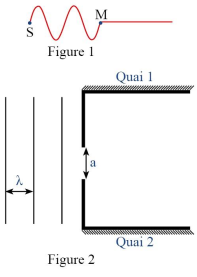
\includegraphics[width=0.19\textwidth]{./img/ex6.png}
  %\end{center}
%\end{wrapfigure}
On réalise le circuit correspondant au schéma-ci après. Un dispositif d’acquisition de
données relié à un ordinateur permet de suivre l’évolution de la tension aux bornes du
condensateur en fonction du temps t.

On déclenche les acquisitions à la fermeture de l’interrupteur $K_1$, le condensateur étant
préalablement déchargé. L’ordinateur nous donne alors $u_c = f(t)$, courbe 1 ci-après.

\begin{center}

	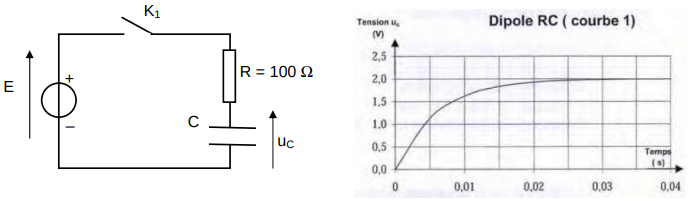
\includegraphics[width=0.8\textwidth]{./img/RC.png}
\end{center}

\textbf{1. LE DIPÔLE RC :}

\begin{tabular}{c|l}
	0,25  & \makecell[l]{\textbf{1.1. }Reproduire le schéma du montage sur la copie et indiquer où doivent être branchées\\ la masse M et la voir d’entrée de la carte d’acquisition pour étudier les
 variations de la \\tension $u_c$ aux bornes du condensateur.\\ Quel est le phénomène
 physique mis en évidence sur l’enregistrement ? }\\

		0,5 & \makecell[l]{\textbf{1.2. }Etablir l’équation différentielle vérifiée par $u_c(t)$.}\\
		0,5 & \makecell[l]{\textbf{1.3. }Trouver les expressions de A et de $\tau$, pour que $u_c(t)=A.(1-e^{-\frac{t}{\tau}})$ soit solution de cette\\équation
		différentielle.}\\

			0,25 & \makecell[l]{\textbf{1.4. }Déterminer la valeur de $\tau$. }\\
			0,25 & \makecell[l]{\textbf{1.5. }Vérifier que la capacité du condensateur est $C=60\mu F$. }\\


\end{tabular}

\section*{Partie 2 :la réponse d’un dipôle RL à un échelon de tension.\dotfill(1.5pts)}
On remplace le condensateur par une bobine d’inductance L et de résistance r selon le
schéma ci-après. L’ordinateur nous permet de suivre l’évolution de l’intensité i du courant en fonction du temps, courbe 2 ci-après. 

\begin{center}

	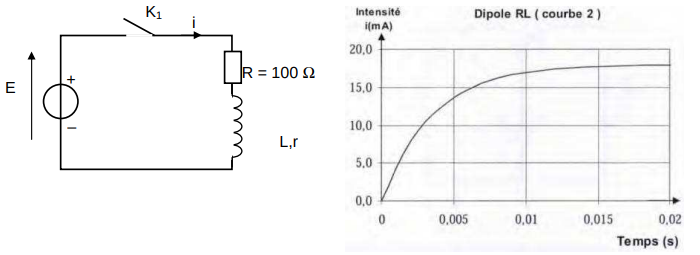
\includegraphics[width=0.8\textwidth]{./img/RL.png}
\end{center}
 La loi d’additivité des tensions appliquée à ce circuit série conduit à l’équation différentielle suivante : $E = (R+ r)i + L.\frac{di}{dt}$  (1)
 \vspace{3cm}

\textbf{2. LE DIPÔLE RL :}

\begin{tabular}{c|l}
	0,25  & \makecell[l]{\textbf{2.1 }Quel est le phénomène physique mis en évidence sur l’enregistrement et quel est l’élément\\ du circuit responsable de ce phénomène ?}\\
	0,25 & \makecell[l]{\textbf{2.2 }Soit I l’intensité du courant électrique qui traverse le circuit, en régime  permanent. \\établir son expression littérale à partir de l’équation (1) en fonction des  grandeurs\\ caractéristiques du circuit. Donner sa valeur numérique et déduire la
 résistance de la bobine. }\\
		0,25 & \makecell[l]{\textbf{2.3. } Quelle est la valeur du courant à la date $t = 0 s$ ? Comment s’écrit alors l’équation
		\\différentielle (1) donnée précédemment ?Montrer qu’à $t = 0 s$, on a $\frac{di}{dt} = \frac{I}{\tau'}$  avec $\tau'=  \frac{L}{R + r}$ \\constante de temps du
 dipôle RL. }\\
			0,25 & \makecell[l]{\textbf{2.4. }Vérifier que $\frac{L}{R+r}$ est homogène à un temps.}\\
			0,5 & \makecell[l]{\textbf{2.5. }Déterminer graphiquement la valeur numérique de $\tau'$ et Vérifier que la valeur\\de  l’inductance de la bobine $L=0,37H$.} 
		\end{tabular}

\section*{Partie 3 :Etude des oscillations dans un circuit RLC série. \dotfill(1,75pts)}
On associe un condensateur de capacité $C = 60 \mu F$ avec la bobine précédente, comme le
montrer le schéma ci-dessous.
Le condensateur est préalablement chargé (interrupteur en position 1). L’enregistrement
des variations de la tension aux bornes du condensateur en fonction du temps commence
quand on bascule K en position 2, courbe 3 ci-après. 

\begin{center}

	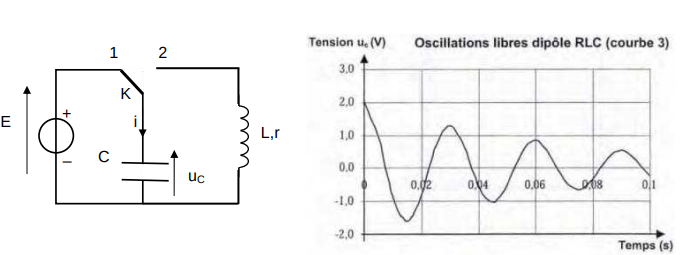
\includegraphics[width=0.8\textwidth]{./img/RLC.png}
\end{center}


\begin{tabular}{c|l}
	0,25  & \makecell[l]{\textbf{3.1 }Quel est le régime d’oscillation mis en évidence par la courbe 3 }\\
	0,5  & \makecell[l]{\textbf{3.2 }Etablir l’équation différentielle vérifiée par la tension $u_c(t).$ }\\
	0,75  & \makecell[l]{\textbf{3.3 }Sachant que la pseudopériode est égale à la période propre,déterminer la valeur de
 \\l’inductance de la bobine. La comparer à celle trouvée précédemment }\\

	0,25  & \makecell[l]{\textbf{3.4 }L’association bobine-condensateur est à la base de la constitution d’oscillateurs qui \\génèrent une tension sinusoïdale constante en fréquence et en amplitude. Ces  oscillateurs\\ sont présents dans de nombreux appareils électriques utilisés dans le domaine des \\télécommunications.
 Comment maintient-on constante l’énergie totale d’un oscillateur électrique ? }\\
	\end{tabular}

\begin{center}
    %\vspace{.60cm}
\hrulefill
\Large{-- Mécanique --}
\hrulefill\\
    \emph{Les  parties sont indépendantes}
\end{center}
\vspace{-1.3cm}
\section*{Partie A :volcan le plus actif au monde.\dotfill(1pts)  }
\begin{wrapfigure}[4]{r}{0.26\textwidth}
	\vspace{-1.5cm}
\begin{center}
  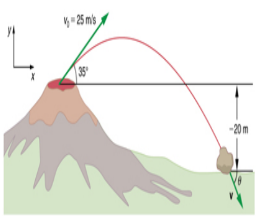
\includegraphics[width=0.26\textwidth]{./img/mecanique.png}
\end{center}
\end{wrapfigure}


Kilauea à Hawaii est le volcan le plus actif au monde. Les volcans très actifs rejettent généralement des roches et de la lave brûlante plutôt que de la fumée et des cendres. Supposons qu’un gros rocher soit éjecté du volcan avec une
vitesse de $25m/s$ et à un angle $\alpha = 35^{\circ}$ au-dessus de l’horizontale, comme indiqué dans la figure(1). 

On donne $g = 9,8m/s$.

\begin{tabular}{c|l}
	
	 0,75 & \makecell[l]{\textbf{1. }La roche heurte le flanc du volcan à une altitude de 20m plus basse que son point de départ. \\.Calculez combien de temps la roche prend pour suivre ce chemin. }\\

	 0,25 & \makecell[l]{\textbf{2. }Quelles sont la valeur et la direction (angle $\theta$) de la vitesse de la roche à l’impact}\\

\end{tabular}


\section*{ Partie B : Etude du mouvement d’un pendule de torsion \dotfill (4pts)}

Cet exercice a pour objectif d’étudier le mouvement d’un pendule de torsion et de déterminer quelques grandeurs liées
à ce mouvement. On dispose d’un pendule de torsion constitué d’un fil métallique , de constante de torsion C et d’une
tige AB homogène fixée en son centre d’inertie G à l’une des extrémités du fil. L’autre extrémité du fil est fixée en un
point O d’un support.
La tige peut effectuer un mouvement de rotation sans frottement autour de l’axe $(\Delta)$ confondu avec le fil métallique.
Le moment d’inertie de la tige AB par rapport à cet axe est $J_0 = \frac{1}{12}ml^2$ avec $l = AB = 20cm$ , $m=600g$ et $OG=L$.

\textbf{l'effet de la longueur du fil.}

\begin{tabular}{c|l}
	
	0,5 & \makecell[l]{\textbf{1.1. }On fixe deux masselottes identiques de masses $\frac{m}{6}$ de part et d’autres de l’axe à une distance d.\\ Calculer la valeur de d pour que $T_0'=\sqrt{2T_0}$. }\\
	0,75 & \makecell[l]{\textbf{1.2 }On fait glissser la tige vers le bas Pour que la longueur du fil augmente par $\frac{L}{4}$, trouver dans\\ ce cas l’expression de $T_0'$ en fonction de $T_0$ sachant que la constante de torsion est inversement \\proportionnel à la longueur du fil .}

 \end{tabular}

 \textbf{l'effet de l'amortissement }

 On enlève les deux masselottes et on fixe à la tige AB, une plaque de masse négligeable qu’on immerge
 partiellement dans un liquide visqueux, qui génère un couple de frottement $M_f = -\alpha.\dot{\theta}$ , où $\alpha$ est une constante positive. On écarte la tige AB de sa position d’équilibre, d’un angle $\alpha = \frac{\pi}{4}$ et on la lâche sans vitesse initiale.
Une carte d’aquisition informatique permet de tracer les variations de l’abscisse de G en fonction du temps.

\begin{tabular}{c|l}
	
	0,5 & \makecell[l]{\textbf{2.1. }Montrer que $\theta$ vérifie l’équation différentielle suivante :$\ddot{\theta} + \frac{\alpha}{J_0}.\dot{\theta} + \frac{c}{J_0}.\theta = 0$ }\\
	0,75 & \makecell[l]{\textbf{2.2. }Montrer que : $\frac{dE_m}{dt} = -\alpha.\dot{\theta}^2$,et commenter le résultat.}\\

	0,75 & \makecell[l]{\textbf{2.3. }Montrer que :$W_{A\rightarrow B}(\vec{F}) = \frac{1}{2}.C(\theta^2_A - \theta^2_B)$), et calculer sa valeur \\entre $t_1 = 1ms$ et $t_2 = 2, 75ms$.  }\\

	0,75 & \makecell[l]{\textbf{2.4 } Calculer $\alpha$ sachant que $\left(\frac{dE_m}{dt}\right)_{t=2,75ms}=2Joule./m.s^{-1}$ }


\end{tabular}


\begin{center}

	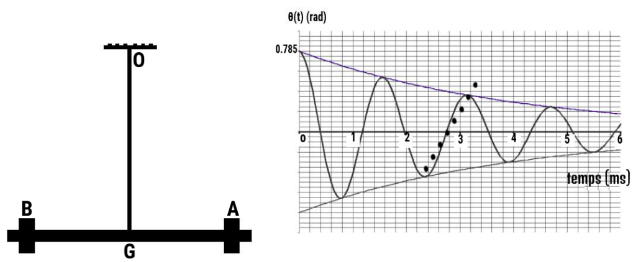
\includegraphics[width=0.8\textwidth]{./img/last.png}
\end{center}




\end{document}
